\RequirePackage[l2tabu, orthodox]{nag}
\documentclass[12pt]{amsart}
\usepackage{fullpage,url,amssymb,enumerate,colonequals,pdfsync,float,mathtools,appendix,float,amsmath,marginnote}
% \usepackage[all]{xy} % for commutative diagrams
%\usepackage{mathrsfs} % for \mathscr (script letters)

\usepackage[marginparwidth=5cm]{geometry}

\usepackage{rotating}
\newcommand*{\isoarrow}[1]{\arrow[#1,"\rotatebox{90}{\(\sim\)}"]}


\usepackage{tikz-cd,graphicx}

\newcommand{\defi}[1]{\textsf{#1}} % for defined terms



\makeatletter
\g@addto@macro\bfseries{\boldmath} % This makes math in section titles bold.
\makeatother

\usepackage{microtype}

%%% \renewcommand{\baselinestretch}{3}   % for triple spacing

\usepackage[
%	draft,
%	colorlinks,
backref,
pdfauthor={Solomon}, % add other authors
%	pdftitle={Paper title goes here},
]{hyperref}
\usepackage[alphabetic,backrefs,lite,nobysame]{amsrefs} % for bibliography

\usepackage{color}


\usepackage[framemethod=tikz]{mdframed}

\newcommand{\isaac}[1]{{\color{magenta} \textsf{$\spadesuit\spadesuit\spadesuit$ isaac: [#1]}}}

\newcommand{\blue}[1]{{\color{blue} #1}}
\newcommand{\magenta}[1]{{\color{magenta} #1}}
\newcommand{\green}[1]{{\color{ForestGreen} #1}}
\newcommand{\dist}{\text{d}}
\numberwithin{figure}{section}
\newtheorem{theorem}{Theorem}


\title{Convolutional Persistence}
\author{EP}
\date{\today}

\begin{document}

	
	\maketitle
	\thispagestyle{empty}
	
	
\section{Overview}
Our focus in this paper is the task of computing functional sublevelset persistence. This is a very general invariant that can be computed for \emph{constructible functions} on \emph{definable sets}, which includes monotonic functions on simplicial complexes. However, we specialize here to the simple, ubiquitous setting where the domain is a cubical grid. This is not strictly necessary for the theory developed here, but significantly simplifies the analysis and computational pipeline, and encompasses many of the applications of interest.\\

To be precise, let $P \subset \mathbb{Z}^d$ be a rectangle inside of the integer lattice, and let $f: P \to \mathbb{R}$ be a function defined on $P$. $P$ can be viewed as the vertex set of an $m$-dimensional cubical complex $K^{m}_{P}$ in which higher-dimensional simplices are given by grid adjacencies, and $f$ can be extended to this complex via the lower-* rule, in which $f(\sigma) = \max_{p \in \sigma}f(p)$, cf. \cite{bleile2021persistent} section 4. Taking the \emph{maximum} here guarantees that a simplex does not appear in a sublevelset filtration until all of its faces do, ensuring that the sublevelsets are valid subcomplexes.\\

There are many areas of application in which the topology of the pair $(K^{m}_{P},f)$ is useful\marginnote{\footnotesize \color{red} Give examples!}. However, there are multiple challenges with computing and using these persistence diagrams:
\begin{itemize}
	\item Persistent homology calculations scale poorly in the size of the input complexes, and hence cannot be effectively applied to many high-resolution images.
	\item Persistent homology calculations are sensitive to outliers, and many real-world images exhibit considerable noise.
	\item Even in the absence of noise, the topological structure in an image may not be evident without some image preprocessing.
	\item Different forms of preprocessing will produce different topological structures in the resultant image. How should we decide which is most relevant for the task at hand?
	\item Functional persistence is not injective, so different images can have the same persistence diagram. This implies a loss of information in any framework that makes decisions on the basis of these diagrams.
\end{itemize}

In this paper, we propose a framework for computing persistence of pairs $(K^{m}_{P},f)$ that addresses all of these concerns simultaneously. This framework is adapted from the concept of a \emph{convolution layer} in modern deep learning. Let $B \subset \mathbb{Z}^d$ be another rectangle, smaller than $P$, and let $g: B \to \mathbb{R}$ be a function on this region; the pair $(B,g)$ acts as a \emph{convolutional filter}. Fix a vector $k = (k_1, \cdots, k_d)$ with $k_i \in \mathbb{N}_{>0}$, corresponding to the \emph{stride} of the convolution. For $v \in \mathbb{Z}^d$, define:
\[(g \ast f)(v) = \sum_{p \in B} g(p)f(p+v \odot k),\]

where $\odot$ is the Hadamard product.Let $R \subset \mathbb{Z}^d$ be the collection of values $r$ such that $B + (r \cdot k) \subseteq P$, which is necessarily also a rectangle. The pair $(R, g \ast f)$ is the output of our convolution. $R$ may be much smaller than the support of $f$, since the various translates of $B$ covering this support are not required to overlap much, if at all. In the degenerate setting where $P$ and $B$ are the same shape, $R$ will consist of a single vertex. For the purposes of computing persistence, we will think of $R$, like $P$, as being the vertex set of a cubical complex $K_{R}^{m}$, and we extend functions on $R$ to the entirety of the cubical complex using the lower-* rule.\\

By analogy with \cite{solomon2021fast,solomon2021geometry}, we propose that the collection of persistence diagrams of the form $PH(K_{R}^{m},g_{i} \ast f)$, for some set of filter functions $\mathcal{G} = \{g_i\}$, is of greater general utility than $PH(K_{P}^{m},f)$. The computational advantages are immediate: when the stride $k$ is large, so that $R$ is much smaller than $P$, we have replaced a single, very expensive calculation with multiple, significantly faster calculations that can be performed in parallel. Moreover, we claim that this approach, which we deem \emph{convolutional persistence}, is more robust and flexible than ordinary persistence, and has superior inverse properties. It is also important to note that the \emph{translation equivariance} of convolutions and the \emph{transational invariance} of persistent homology work well together.\\

%It is also important to note that convolution is \emph{translation equivariant} and persistence is \emph{translation invariant}, so their composition is translation invariant.\\

\emph{Stability and robustness} are not hard to justify. If $g$ is a filter function with $\|g\| \leq 1$, then $\|g \ast f_1 - g \ast f_2 \| \leq \|f_1 - f_2\|$ by the Cauchy-Schwarz inequality, providing stability. A classical example is the \emph{box-smoothing} filter $g(p) = \frac{1}{|B|}$. Such smoothing filters also do a good job of diminishing the impact of outliers. \emph{Flexibility} is also immediate, since the collection of filters $\mathcal{G}$ can be curated for the task at hand, and can be learned using a training dataset.\\

Let us now demonstrate injectivity. For a fixed function $f:P \to \mathbb{R}$ and stride vector $k$, we can obtain a mapping $\iota_{f}$ of the rectangle $R$ into $\mathbb{R}^{|B|}$ by sending every point $r \in R$ to the vector $\{f(b + k \odot r) \mid b \in B\}$. This is technically a set, rather than a vector, but it becomes a vector after fixing an order on the elements of $B$. Such a mapping can be extended linearly to the entire cubical complex $K_{R}$ built on top of $R$. Let us suppose that $\iota_{f}$ is injective on the $m$-skeleton $K_{R}^m$, so that $\iota_{f}(K_{R}^m)$ has the structure of a simplicial complex isomorphic to $K_{R}^m$. Then for a function $g: B \to \mathbb{R}$, viewed also as a vector $\vec{g} \in \mathbb{R}^{|B|}$, and threshold value $t$, the sets $\{\sigma \in K_{R}^{m} \mid g(\sigma) \leq t\}$ and $\{\sigma \in \iota_{f}(K_{R}^m) \mid \sigma \cdot \vec{g} \leq t \}$ are homeomorphic. See Figure \ref{fig:embedding} for a visual schematic. This means that the persistence diagram $PH(K_{R}^m,g \ast f)$ is identical to the persistence diagram $PH(\iota_{f}(K_{R}^m),\langle g, \cdot \rangle)$. If $g$ is varied over the unit sphere in $\mathbb{R}^{|B|}$, the set of diagrams $PH(\iota_{f}(K_{R}^m),\langle g, \cdot \rangle)$ is known as the \emph{Persistent Homology Transform} which is known to be injective, see \cite{turner2014persistent,ghrist2018persistent,curry2018many}. Thus, the collection of persistence diagrams of the form $\{PH(K_{R}^m, g \ast f) \mid g : B \to \mathbb{R}\}$ is injective. Note that the distinction between using all functions $g: B \to \mathbb{R}$, or only normalized functions lying on the sphere, is immaterial, as persistent homology transforms trivially under rescaling of the height function, so these two invariants determine one another.\\ 

%\marginnote{\footnotesize \color{red} Cite PHT papers}
\begin{figure}
	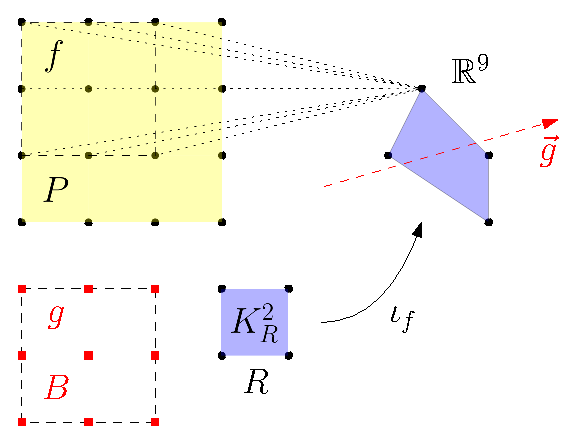
\includegraphics{embedding}
	\caption{The function $f$ is defined on the $4 \times 4$ grid on the top left. The box $B$ is $3 \times 3$, and using a $(1,1)$-stride there are four ways of laying $B$ over the domain of $f$, so that $R$ is a $2 \times 2$ grid. We can map the vertices of $R$ into $\mathbb{R}^9$ by associating each vertex of $R$ with its corresponding translate of $B$, and then taking as coordinates the values of $f$ in that translate. This extends linearly to a map $\iota_{f}$ from the complex $K_{R}^2$ in $\mathbb{R}^9$, which here is shown to be an embedding.}
	\label{fig:embedding}
\end{figure}

The above proof of injectivity for \emph{convolutional persistence} relies on $\iota_{f}:K_{R}^{m} \to \mathbb{R}^{|B|}$ being injective. We claim that this is generically the case whenever $\kappa = \Pi_{i}k_i > 2m$. Indeed, let $B^{*} \subseteq B$ consist of those elements in the top-left $k_1 \times k_2 \times \cdots k_d$ corner of $B$. The various translates $B^{*} + (k \odot r)$ are all disjoint subsets of $P$. We can thus view the vertices $\{f(b + k \odot r) \mid b \in B\}$ of $\iota_{f}(K_{R}^m)$ as having at least $\kappa$ degrees of freedom, and this can be made more precise by projecting the embedding on to the coordinates corresponding to $B^*$. We now want to show that if we choose a collection $S$ of points in $\mathbb{R}^{M}$ for $M > 2m$, and build the complete $m$-dimensional complex on top of these points, we will generically never have nontrivial intersections of disjoint simplices. To see why this is the case, let $\sigma$ and $\tau$ be simplices corresponding to disjoint subsets $S_{\sigma}$ and $S_{\tau}$ of $S$. If $\sigma$ and $\tau$ intersect, then their union is contained in an affine subset of $\mathbb{R}^M$ of dimension $(\dim \sigma + \dim \tau)$. Now, whenever $M > \dim \sigma + \dim \tau$, a collection of at least $(\dim \sigma + \dim \tau + 2)$ points generically does not lie on an affine subset of dimension $(\dim \sigma + \dim \tau)$. Since $M > 2m \geq \dim \sigma + \dim \tau$, and $|S_{\sigma} \cup S_{\tau}| = |S_{\sigma}| + |S_{\tau}| = (\dim \sigma + 1) + (\dim \tau + 1) = \dim \sigma + \dim \tau + 2$, we see that the intersection of $\sigma$ and $\tau$ is not generic.\\

What we have just shown is that having a large stride vector, in addition to providing computational speedups by lowering the resolution of the resultant grid, also provides generic injectivity for persistence of higher-dimensional data complexes.\\ 

Now, what we have described above is persistence with a single convolutional layer. One can extend this construction by convolving the collection $\{(R, f \ast g) \mid g \in \mathcal{G}\}$ using a new rectangle $B'$ and collection $\mathcal{H}$ of filter functions $h: B' \to \mathbb{R}$, and \emph{then} compute persistence. This pipeline remains injective, because the collection $\{(R, g \ast f) \mid g: B \to \mathbb{R}\}$ determines the function $f$ (this is trivial, consider characteristic functions of pixels in $B$), so the two-layer convolutional persistence is a composition of two injective operations, where we are now taking the sets $\mathcal{G}$ and $\mathcal{H}$ to consist of \emph{all possible filters}. We might also consider introducing a non-linear activation between the convolutional layers, following more closely the structure of a CNN.\\

An alternative convolutional pipeline is to do a convolutional with a small stride, so that the resulting image has the same resolution as the original, and then apply a pooling later. This mirrors more closely the structure of a modern CNN. Note that this pipeline also enjoys an inverse result, provided that the corresponding embedding is injective on the input cubical complex\marginnote{\footnotesize \color{red} Make rigorous}.\\

In practice, of course, we are not interested in considering infinitely many filter functions. Indeed, learning tasks require invariants to \emph{retain} features that are important to classification or regression, and \emph{forget} features that are not. Thus, we will want to pick $\mathcal{G}$ appropriately. There are many ways for this choice to be made:
\begin{enumerate}
	\item Take $\mathcal{G}$ to consist of a collection of popular filters in image processing, like blurring, sharpening, and boundary detection.
	\item Take $\mathcal{G}$ to consist of Klein filters, as identified by Carlsson et al.
	\item Take $\mathcal{G}$ to consist of eigenfilters identified via PCA on the set of patches of images in the training set.
	\item Incorporate convolutional persistence in a deep learning pipeline and learn $\mathcal{G}$ to minimize a chosen loss function.
\end{enumerate}

For the third point above, note that the inverse results for the PHT do not require all sphere directions when the shape in question sits inside a low-dimensional space of Euclidean space. Thus, it makes sense to ignore filters orthogonal to the space of image patches in question.\\

%and this introduces an important tradeoff in convolutional optimization. When the convolutional rectangle $R$ and the stride $k$ are large, the decrease is resolution is quite substantial, yet the number of free parameters to be learned is large. This makes optimization difficult, but also allows for more sophisticated filters. Conversely, when the rectangle and stride are small, there is a more minor decrease in resolution, but a simpler optimization task. As for learning more complicated filters, this is still possible when there are multiple convolutional layers.\\ 
 
  
{\bf Prior Work:} This is not the first work where convolutions and persistence have been investigated. They were considered in APE I. They are also mentioned in ``PLLay: Efficient Topological Layer based on Persistence Landscapes". What makes this work unique is that it extends APE I by considering general convolutional layers, rather than noisy box smoothing, and it extends the PPLay paper by considering non-deep-learning approaches to convolutional persistence, focusing on the ability of convolutionals to speed up persistence calculations, rather than just extract more features for a CNN, and investigating more deeply into questions of injectivity and optimization.\\

{\bf Goal:} The goal of this paper is to verify or rule out the following conjectures: 
\begin{itemize}
	\item Convolutional persistence can achieve reasonable accuracy on complex learning tasks for shapes defined by height functions over cubical grids.
	\item Convolutional persistence can be incorporated into other deep learning pipelines and provide some improvement in accuracy.
\end{itemize}


{\bf Experimental Pipeline:}
\begin{enumerate}
	\item In the first phase of the pipeline, we consider the digits dataset, which is small enough that ordinary persistence calculations are very fast. Thus, the role of this phase is to understand how convolutions improve the utility of persistence features. The first step of this phase is to see how standard ML models perform on digit classification based on cubical persistence features. We can then enrich this featurization using different choices of fixed filters $\mathcal{G}$, as outlined above, and see the impact this has on performance. The fundamental question here is whether or not reasonably good performance can be achieved through convolutional persistence. 
	\item The second phase of the pipeline is to try and learn the filters $\mathcal{G}$ using a deep learning architecture. This will require more work than choosing fixed filters as above.
	\item The third phase is to extend the experiments above to larger data sets, like CIFAR, where the downsampling aspect of the convolutions will also be of importance.
\end{enumerate}


\bibliography{convpersbib}
%
%
%$K$ be a pure $d$-dimensional simplicial complex, meaning that every simplex in $K$ is the face of some $d$-simplex. Let $f: K \to \mathbb{R}$ be a function on the top-dimensional simplices of $K$ extended to all of $K$ via the upper-* filtration: $f(\sigma) = \min \{f(\tau) \mid \sigma < \tau \mbox{ and } \operatorname{dim}(\tau) = d\}$. A very general example is when $K$ is a finite grid complex in $\mathbb{R}^d$, and $f:K \to \mathbb{R}$ records the values of some image defined on the pixels or voxels of $K$.


%a \emph{cubical complex} $K$ arising as the intersection of the integer grid complex $\mathbb{Z}^d$ in $\mathbb{R}^d$ with a rectangle of the form $\Pi_{i=1}^{d}[a_i,b_i]$, where $a_i, b_i \in \mathbb{Z}$. We will call such a complex $K$ a \emph{finite integer grid}. Given a real-valued function $f$ on the $d$-dimensional cells of $K$, this naturally extends to all of $K$ by asserting that $f(\sigma) = \min \{f(\tau) \mid \sigma < \tau \mbox{ and } \operatorname{dim}(\tau) = d\}$. When $d=2$, such a pair $(K,f)$ is simply an image defined over a rectangular array of pixels, and for $d=3$ we have an image defined over a rectangular array of voxels. More generally, we might allow $f$ to take values in $\mathbb{R}^k$ for $k>1$, in which case we have an image with multiple \emph{channels}.\\

%That is, we consider covering $K$ with translates of a fixed subgrid $L$, and denote the dual of the \v{Cech} complex of the cover by $K/L$. If, moreover, we equip $L$ with a function $g: L \to \mathbb{R}$, we have a recipe for producing a function on the top-dimensional cells of $K/L$, which works as follows: Let $U \subset K$ be a set in the cover of $K$ by translates of $L$, which gives rise to a top-dimensional simplex $[U]$ in $K/L$, and define $f \ast g$ on $[U]$ to be $\sum_{\tau \in U} f(\tau)g(\tau)$, where the sum is taken over $d$-dimensional simplices in $U$.  




\end{document}